\documentclass[11pt, oneside]{amsart}   	% use "amsart" instead of "article" for AMSLaTeX format
\usepackage{geometry}                		% See geometry.pdf to learn the layout options. There are lots.
\geometry{letterpaper}                   		% ... or a4paper or a5paper or ...
%\geometry{landscape}                		% Activate for rotated page geometry
%\usepackage[parfill]{parskip}    		% Activate to begin paragraphs with an empty line rather than an indent
\usepackage{graphicx}				% Use pdf, png, jpg, or eps§ with pdflatex; use eps in DVI mode
								% TeX will automatically convert eps --> pdf in pdflatex
\usepackage{amssymb}
\usepackage{amsmath}
\usepackage{hyperref}

%SetFonts
\usepackage[utf8x]{inputenc}
\usepackage[T1]{fontenc}
\usepackage{lmodern}


\nonstopmode
%----macros begin-----------------------------------------------------------------------------------
\usepackage{graphicx}
\usepackage{color}

\def\conv{\mbox{\textrm{conv}\,}}
\def\aff{\mbox{\textrm{aff}\,}}
\def\B{\mathbb{B}}
\def\N{\mathbb{N}}
\def\E{\mathbb{E}}
\def\R{\mathbb{R}}
\def\Z{\mathbb{Z}}
\def\v#1{{\bf #1}}
\def\p#1{{\bf #1}}
\def\T#1{{\bf #1}}
\def\vet#1{{\left(\begin{array}{ccccccc}#1\end{array}\right)}}
\def\mat#1{{\left(\begin{array}{ccccccc}#1\end{array}\right)}}

\def\lin{\mbox{\rm lin}\,}
\def\aff{\mbox{\rm aff}\,}
\def\pos{\mbox{\rm pos}\,}
\def\cone{\mbox{\rm cone}\,}
\def\conv{\mbox{\rm conv}\,}

%----macros end-----------------------------------------------------------------------------------


% rules for for inputed tables
% the
\usepackage{siunitx}
\usepackage{booktabs}

%alternative rules for tables
%\newcommand{\toprule}{\hline}
%\newcommand{\midrule}{\hline}
%\newcommand{\bottomrule}{\hline}
%\newcommand{\specialrule}{}

%SetFonts



\title{Algebraic filtering of surfaces from medical images with Julia}
\author{Miroslav Jirik and Alberto Paoluzzi}
\date{}							% Activate to display a given date or no date

\begin{document}
\maketitle

\begin{abstract}
In this paper we introduce a novel algebraic \textsc{lar-surf} filter, well founded on algebraic topology methods, to extract and smooth the boundary surface of any subset of voxels arising from  segmentation of a 3D medical image. The input is defined as a \emph{chain}, i.e.~as a vector from a linear space of 3-chains, represented in coordinates as a sparse binary vector. The output is produced by a linear mapping between spaces of 3- and 2-chains through the boundary operator $\partial_3:C_3 \to C_2$.  In particular, when the input set of voxels is either not (4-)connected, or contains one or more empty regions inside, \textsc{lar-surf} generates a non connected set of closed surfaces, i.e.~a set of 2-cycles---using the language of algebraic topology. The only data structures used by this approach are sparse arrays with one or two indices, i.e.~sparse vectors and matrices. This work is based on LAR (Linear Algebraic Representation) methods, and is implemented in Julia language, natively supporting parallel computing on hybrid architectures.
\end{abstract}

\tableofcontents

%\section{}
%\subsection{}

\section{Introduction}\label{sec:intro}


Isosurface extraction produces geometric model of surface 
 from volumetric data is important in many aplications. It is often used for indirect visualization of the medical data or for flow modeling \cite{Rohan2018a}.
 
 
The most popular algorithm used for surface extraction is probably Marching Cubes (MC). The algorithm was described by Lorentsen and Cline \cite{Lorensen1987} in 1987. Survey of Marching Cubes algorthm has been published in 2006 \cite{Newman2006}. The algorithm is based on considering the cube defining volume. Each corner vertex of the cube is related to input volumetric data. MC traverse the data and constructs the surface by using lookup table of different triangular faces depending on different patterns of the cube.  Main disadvantages of this method are time requirements, ambiquity and holes generation. Some of them were discoverd shortly after the algorithm was introduced. 
Marching Cubes. In 1991 Nielson and Hamman described Asymptotic Decider to solve the ambiguity problem on the faces of the cube.  Natarajan noted that the ambiguity problem also occurs in cubes \cite{Natarajan1994}. In 1995 Chernyaev extended the number of cases to 33 \cite{chernyaev1995marching}. More recently the algorithm was updated by Custodio to   enhance the quality of triangulation \cite{Custodio2019}. 

The alternative methods have been deveoloped including method for surface extraction using particle attraction system was described by Crossno and Angel in \cite{Crossno2002} and method processing on a graph that tracks cell face adjacencies is described in \cite{Lachaud2000}. The parallel algorithms for surface extraction are discussed in \cite{Bajaj2004}.





\section{Background}\label{sec:background}


\subsection{Representation Schemes}\label{sec:aaaa}

A \emph{representation scheme} for solid modeling is a mapping between a space of mathematical models and a space of symbolic representations, often generated by a formal grammar.
Solid pointsets (i.e., `$r$-sets') are defined~\cite{Requicha:1980:RRS:356827.356833} as compact (bounded and closed) regular and semianalytic subsets of the $d$-space. A large number of representation schemes were defined in the past forty years, including the two main classes of (a) \emph{boundary representations} (`$B$-reps'), where the solid model is represented through a representation of its boundary elements, i.e.~faces, edges and vertices, and (b) \emph{decompositive/enumerative representations}, that are a decomposition of either the object or the embedding space, respectively, into a well-defined \emph{cellular complex}. In particular, a boundary representation provides a cellular decomposition of the object's boundary into \emph{cells} of dimension zero (vertices), one (edges), and two (faces). Medical imaging can be classified as \emph{enumerative representation} of cellular decompositions of organs and tissues of interest, in particular, as subsets \emph{of 3D volume elements} (voxels) from the 3D image. 


\subsection{Linear Algebraic Representation}\label{sec:aaaa}

The \emph{Linear Algebraic Representation} (\textsc{lar})~\cite{Dicarlo:2014:TNL:2543138.2543294} aims to represent the \emph{chain complex}~\cite{TSAS} generated by a piecewise-linear geometric complex embedded either in 2D or in 3D. In few words, it gets a minimal characterization of geometry and topology of a cellular complex, i.e.~the embedding mapping $\mu : C_0 \to \E^d$ of 0-cells (vertices), as well a description of $(d-1)$-cells as subsets of vertices, and is able to return the whole chain complex 
\[ 
C_\bullet = (C_p, \partial_p) := 
C_3 \ 
\substack{
\delta_2 \\
\longleftarrow \\[-1mm]
\longrightarrow \\
\partial_3 
}
\ C_2 \ 
\substack{
\delta_1 \\
\longleftarrow \\[-1mm]
\longrightarrow \\
\partial_2 
}
\ C_1 \ 
\substack{
\delta_0 \\
\longleftarrow \\[-1mm]
\longrightarrow \\
\partial_1 
}
\ C_0 .
\] 
and, in particular, any basis for linear chain spaces $C_p$, and any linear
boundary/coboundary map \(\partial_p\) and
\(\delta_p=\partial_{p+1}^\top\) between them. The \emph{domain} of \textsc{lar} is the set of \textbf{chain complexes} generated by cell $d$-complexes ($2\leq d\leq 3$). The computer \emph{representations} of \textsc{lar} are \textbf{sparse binary matrices} to represent both the operators and the chain bases. Note that in algebraic topology a $p$-chain is defined as a linear combination of $p$-cells with scalars from a field. When the scalar coefficients are from $\{-1, 0, +1\}$, a chain may represent \emph{any (oriented) subset of cells} from the cellular complex. 

We may therefore get the $(p-1)$-boundary $\partial_p \gamma_p$ of \emph{any} $p$-chain $\gamma_p$, by multiplication of the coordinate representation $[\partial_p]$ of the boundary operator times the coordinate representation $[\gamma_p]$ of the chain in terms of such scalars, i.e.~by a  matrix-vector product $ [\partial_p] [\gamma_p] $.

It is easy to understand that the \textsc{lar} representation scheme is very expressive, i.e.~that it  has a large domain,  including collections of: line segments, quads, triangles, polygons, meshes;  pixels, voxels, volume images; B-reps, enumerative and decompositive representations of solids. 
In this paper we apply \textsc{lar} methods to computation of boundary representations of solid models from segmentation (labeling) of 3D medical images.

\subsubsection{Construction of $\partial_d$ boundary matrix}

Once fixed an ordering for all the cells (vertices, edges, pixels, and voxels), i.e.~for 0-, 1-, 2-, and 3-elements of a cell partitioning of a 3D image, i.e., once fixed the $p$-bases for linear spaces $C_p$ of $p$-chains $(0\leq p\leq d)$, we call $M_p = (m_{i,j})$ the \emph{characteristic matrix} of the $p$-basis, expressed as subsets of 0-cells, where  we have that $m_{i,j}=1$ iff the $j$-th $0$-cell belongs to the $i$-th $p$-cell, and $m_{i,j}=0$ otherwise.  

Note that, by computing the (sparse) matrix product $(M_{p-1} M_{p}^t) = (n_{i,j})$, with $n_{i,j} = \sum_{k} m_{i,k}m_{k,j}$, we get for each $n_{ij}$ the \emph{number of vertices} shared by $c_{p-1}^i$ and $c_{p}^j$. When this number equates the cardinality of $c_{p-1}^i$, this elementary chain is contained on the boundary of $c_{p}^j$. In a 3D image, with cubic 3-cells and squared 2-cells, everywhere we get $n_{i,j}=4$, we may state $c_{2}^i\subset\partial c_{3}^j$. In this case, by looking in each $j$ column of $M_{2} M_{3}^t = (n_{i,j})$, we have exactly \emph{six rows} where  $n_{i,j} = 4$. 

Finally, consider the linear graded boundary operator $\partial_p : C_p \to C_{p-1}$. As such, it contains by columns the representation of domain basis elements, expressed as linear combination of the basis elements of the range space. Therefore, the operator matrix $[\partial_d]$ is readily obtained by setting $[\partial_d](i,j)=1$ iff $n_{i,j}=4$ and $[\partial_d](i,j)=0$ otherwise.  Of course, it will contain six non-zero elements for column.  It may be worth to remember that every 3-cell (voxel) has exactly six 2-faces. 

It is possible to show that all the interesting relation of incidence/adjacency between cells of different dimensions can be both computed and efficiently queried by pairwise computing some products, with one of terms possibly transposed, of the two boundary and coboundary operator matrices $[\partial_p]$ and $[\delta_p] = [\partial_p^\top] = [\partial_p]^t$. We may also show that such matrices are \emph{very sparse}, with their sparseness growing rapidly with the dimensions (see Section~\ref{sec:block}). The pattern of non-zeros in matrix $[\partial_3]$ corresponding to a brick of shape $(4,4,4)$ is given in Figure~\ref{fig:boundary_matrix_4x4x4}.

\begin{figure}[htbp] %  figure placement: here, top, bottom, or page
   \centering
   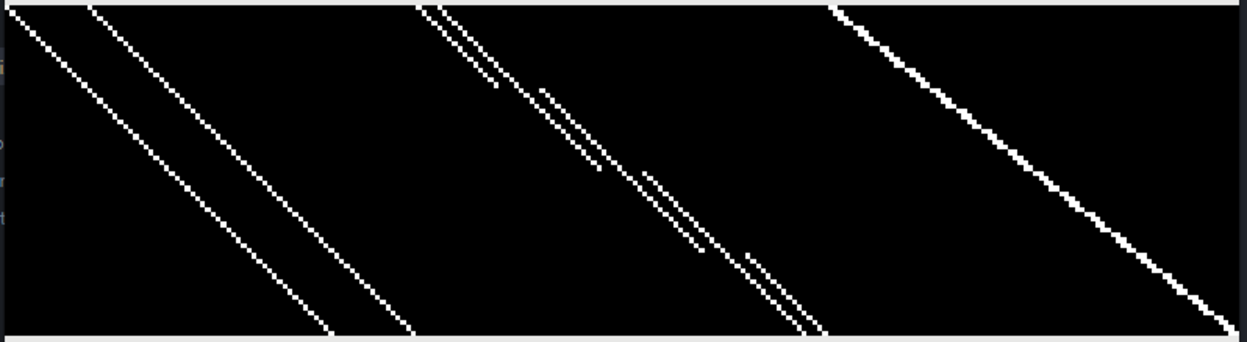
\includegraphics[width=0.75\linewidth]{figs/boundary_matrix_4x4x4.pdf} 
   \caption{A binary image of the coboundary operator  $\delta_2 = \partial^\top : C_2 \to C_3$, built for small 3D images with shape $(4,4,4)$. Note that the number of rows equates the cardinality $4\times 4\times 4 = 64$ of the voxel set; the number of columns is $d\,n\,(1+n)^{d-1} = 3\times 4\times 25 = 300$. Of course, the number of non-zeros per row (cardinality of single voxel facets) is six.}
   \label{fig:boundary_matrix_4x4x4}
\end{figure}

\subsection{Multiindices from Cartesian indices}\label{sec:aaaa}

In order to utilize the topological algebra shortly recalled in this paper, we need to explicitly sort the cells of the various dimensions into linearly ordered sequences, possibly according to the linear order their information is linearly accommodated in computer storage. 

\subsection{Taubin Smoothing}\label{sec:aaaa}






\section{Block-parametric design}\label{sec:filter}

\subsection{Block decomposition}\label{sec:bbbb}

We assume that medical devices produce 3D images with lateral dimensions that are integer multiples of some powers of two, like 128, 256, 512, etc.
Any cuboidal portion of image is completely determined by the Cartesian indices of its voxel of lowest and highest indices, and extracted by multidimensional array \emph{slicing} as $Image([\ell_x$:$h_x, \ell_y$:$h_y, \ell_z$:$h_z])$.

For the sake of simplicity, we assume a common size on the three image axes, and the corresponding image portion $B$, called \emph{block}, as a function of its element of the  lowest  block  coordinates $i,j,k\in\N$ and of block dimension $n$:
\[
B(i,j,k,n) := Image([in\mbox{:}in+n, jn\mbox{:}jn+n, kn\mbox{:}kn+n]) 
\]

\begin{figure}[htbp] %  figure placement: here, top, bottom, or page
   \centering
   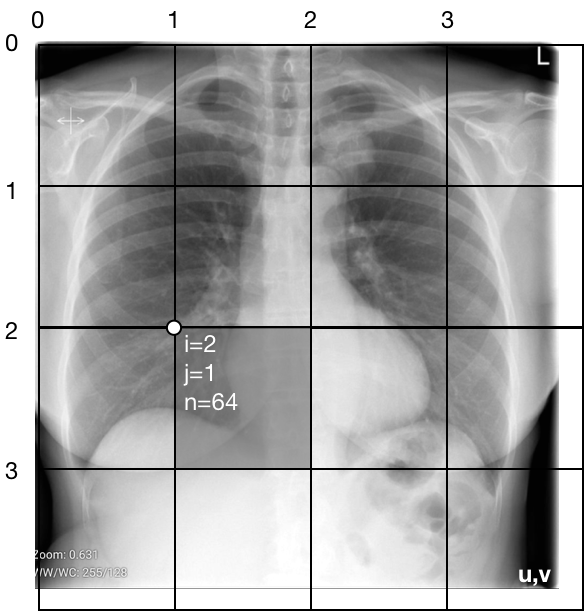
\includegraphics[width=0.5\linewidth]{figs/blocks} 
   \caption{A possible block partitioning of a radiologic image. The evidenced 2D block, of size $n^d=64^2$, is sliced as $B([2,1,64]) = Image([128:172],[64:128)]$}
   \label{fig:blocks}
\end{figure}


Figure~\ref{fig:blocks} shows the block decomposition in a 2D image, with positive integer $u,v$ lateral sizes of image. Note that block sides do not necessarily correspond to image edges. 


\subsection{Block operator }\label{sec:block}

\paragraph{Chain coordinates }\label{sec:bbbb} 
We are going to treat each image block independently from each other. Hence we map each image subspace $B(i,j,n)$ to the linear \emph{chain} space $C_2$ of dimension $n\times n$, using coordinate vectors $c_{h,k}\in \B^{n\times n} := \{0,1\}^{n\times n}$, where the basis element $c = c_{h,k} \in C_2$ is mapped via Cartesian-to-linear map to the Boolean vector 
\[
Image(h,k) \mapsto c_{h,k} := [0 \cdots 0\ 1\ 0 \cdots 0] \in \B^{n\times n}
\]
for each $0\leq h,k \leq n$, and where the (single) unit element is in position $nk + h \leq n\times n$.

Therefore, each pixel (or voxel) in a block image will be seen as a basis Boolean vector in $C_2$, and each subset of image elements, as the corresponding Boolean vector in $C_2$, with many ones as the cardinality of the subset.

\paragraph{Boundary operator }\label{sec:bbbb} For a fixed block size $n$, the boundary operator $\partial_d : C_d\to C_{d-1}$, with $d\in\{2,3\}$, will be constructed once and for all using the algorithm given in~\cite{}, and inlined in the generated boundary extraction code.

It is easy to see that the operator's matrix $[\partial_d]$ is \emph{very sparse}, since it contains $2\times d$ non-zero elements (ones) for each column (of length $n^d$), i.e.~4 ones and 6 ones for the 2D and 3D case, respectively. In fact the matrix of a linear operator between linear spaces contains by columns the basis element of the domain space, represented in the target space. In our case, the former is an image element (2-cube or 3-cube), represented as the chain of its boundary---i.e. either a 1-cycle of 4 edges, or  a 2-cycle of 6 faces, respectively.  

The number of rows of $[\partial_d]$ equates the dimension of the linear space $C_{d-1}$, i.e.~the number of $(d-1)$-cells---elementary $(d-1)$-chains---in the cellular partition of the image. To compute their number, we act in two steps. (a) First we map one-to-one the $n^d$ $d$-cells with $d$ adjacent $(d-1)$-cells, so getting $d\,n^d$ distinct basis elements of $C_{d-1}$. (b) Then we complete this bases by adjoining $n^{d-1}$ boundary elements for each of the $d$ dimensions of the image, so providing further $d\,n^{d-1}$ basis elements for $C_{d-1}$. The dimension of $C_{d-1}$, and therefore the number of rows of $[\partial_d]$ matrix is $d\,(n^{d-1}+n^{d}) = d\,n\,(1+n)^{d-1}$. The number of column equates the number of basis elements of $C_d$, i.e.~the number $n^d$ of block elements.

\paragraph{Sparsity and size of boundary matrix }\label{sec:bbbb} 

As we have seen, we have $2d$ non-zero elements for each column of $[\partial_d]$, so that their total number is $2d\,n^d$. The number of matrix element is $d\,n\,(1+n)^{d-1} \times n^d$, giving a ratio of 
\[
\frac{\mbox{non-zero\ elements}}{\mbox{total\ elements}} = 
\frac{2d\times n^d}{d\,n\,(1+n)^{d-1} \times n^d} =
\frac{2}{n+n^d}
\]
Using sparse matrices in CSC (Compressed Sparse Column) format we get a storage size:
\[
mem([\partial_d]_{n^d}) = 2\times \#\mbox{nzero} + \#\mbox{columns} = 2\times 2d\,n^d + n^d = (4d+1)n^d.
\]
In conclusion, for block size $n=64$, the matrix $[\partial_d]$ requires for 2D images $9\times 64^2=36,864$ memory elements, and for 3D images $13\times 64^3=3,407,872$ memory elements. Counting the bytes for the standard implementation of a sparse binary matrix (1 byte for values and 8 bytes for indices) we get $(18d+8)n^d$ bytes, giving $176$\,KB for 2D and $15.872$\,MB for 3D.

\subsection{Block boundary mapping}\label{sec:bbbb}

Here we refer directly to the 3D case.
Let us call \emph{segment} the bulk content $S$ of interest within the input 3D image of size $(u,v,w)$. We aim to compute the segment boundary $\partial_3 S$. 
First we set the size $n$ of the block, in order to decompose the input $Image(u,v,w)$ into a fair number 
\[
M = \ceil{u/n} \times \ceil{v/n} \times \ceil{w/n} \simeq \frac{uvw}{n^3}
\] of blocks. 
Then we consider each image portion $c_{i,j,k} = S\cap B(i,j,k,n)$ and compute its (binary) coordinate representation  $[c]_{i,j,k}\in C_3(n,n,n)$. This one is a sparse binary vector of length $n^3$. Then assemble the $M$ representations $c$ of segment portions into a sparse binary matrix $\T{S}$, of dimension $n^d \times M$. Finally compute a matrix $\T{B}$ of boundary portions of $S$, represented by columns as chain coordinate vectors in $C_2$:
\[
\T{B} = [\partial_3(n)]\, \T{S}.
\]
where the boundary matrix has dimension $d\,n\,(1+n)^{d-1} \times n^d$.
Of course, the $\T{B}$ sparse matrix has the same column number $M$ of $\T{S}$, because each column contains the boundary representation of the corresponding $S\cap Box_{i,j,k}{i,j,k}$, and the number of rows of the operator, equal to the dimension of the linear space $C_2$.

\paragraph{Embedding}
A final computational step is needed, in order to embed the 2-chains in Euclidean space $\E^3$ and to assemble the whole resulting surface. In particular, we need to compute the \emph{embedding function} $\mu : C_0 \to \E^3$, where $C_0$ is the space of 0-chains, one-to-one corresponding to the vertices of the extracted surface. The simplest solution is to associate  four 0-cells to each 2-cell of the extracted surface, i.e.~to each non-zero entry in every column of \T{B}.  The $\mu$ function  can be computed by identifying, via  element position in the column, a triple of integer values $0\leq x\leq u$, $0\leq y\leq v$, and $0\leq z\leq w$ for each vertex of the 2-cell.  The mapping can be implemented using a dictionary, that will store the inverse coordinate transformation used at the beginning, i.e.~the one from linear to Cartesian coords, in order of not duplicating the output vertices.   

\paragraph{Surface assembling}

All boundary surface subsets $B_{i,j,k}(S) = \partial_3 S \cap \mbox{Box}_{i,j,k}$, provided by  columns of $\T{S}$, are embedded in the same coordinate space. In formal terms: 
\[
\texttt{Lar}(S) := (\texttt{Geom}(S), \texttt{Top}(S)) = (\texttt{V}, \texttt{CV}),
\]
where, with respect to the \emph{chain complex} $C_3\to C_2\to C_1\to C_0$ induced by the input image $Im$ and segment $S_{i,j,k}$, we get
\begin{align}
\texttt{Geom} &:= \mu(C_0(_{i,j,k})) = \texttt{V},
\\
\texttt{Top} &:= C_3(S) = \T{S} \mapsto \texttt{CV}.
\end{align}
and
\begin{align}
\texttt{Lar}(B_{i,j,k}) &:= (\texttt{Geom}, \texttt{Top}) = (\texttt{W}, \texttt{FW}),
\\
\texttt{Geom} &:= \mu(C_0(B_{i,j,k})) = \texttt{W} \subset \texttt{V},
\\
\texttt{Top} &:= C_2(B_{i,j,k}) = \T{B}_{i,j,k} \mapsto \texttt{FW} \subset \texttt{FV}.
\end{align}


A translation transformation applied to each vertex subset $\texttt{W}_{i,j,k}$ with translation  vector $\v{t} = [i,j,k]$ will therefore move it in the final space position, so finally giving
\[
\texttt{Lar}(B) = \oplus_{i,j,k}\texttt{Lar}(\partial_3 S_{i,j,k})) = \oplus_{i,j,k}(\texttt{W}, \texttt{FW}) .
\]


\subsection{Block-level parallelism}\label{sec:bbbb}

In the computational pipeline introduced in this paper, several steps can be efficiently performed in parallel at image-block level, depending on the embarassingly data parallel nature of the problem. In particular, little effort is needed to separate the problem into a number of parallel tasks $S_{i,j,k}$, using multiarray slicing. The granularity of parallelism, depending on the block size $n$, is further enforced by the computation of a single boundary matrix $[\partial_d(n)]$, in turn depending on $n$, so that the initial communication cost of broadcasting the matrix to nodes can be carefully controlled, and finely tuned depending on the system architecture. The whole approach is appropriate  for SIMD hybrid architectures of CPUs and GPUs, since only the initial block setup of boundary matrix and image slices, as well the final collection of computed surface portions, require inter-process communication.






\subsection{Julia implementation}\label{sec:implementation}


\subsubsection{Code optimization}\label{sec:optimization}


\subsubsection{Performance analysis}\label{sec:analysis}



\section{Examples}\label{sec:examples}

% 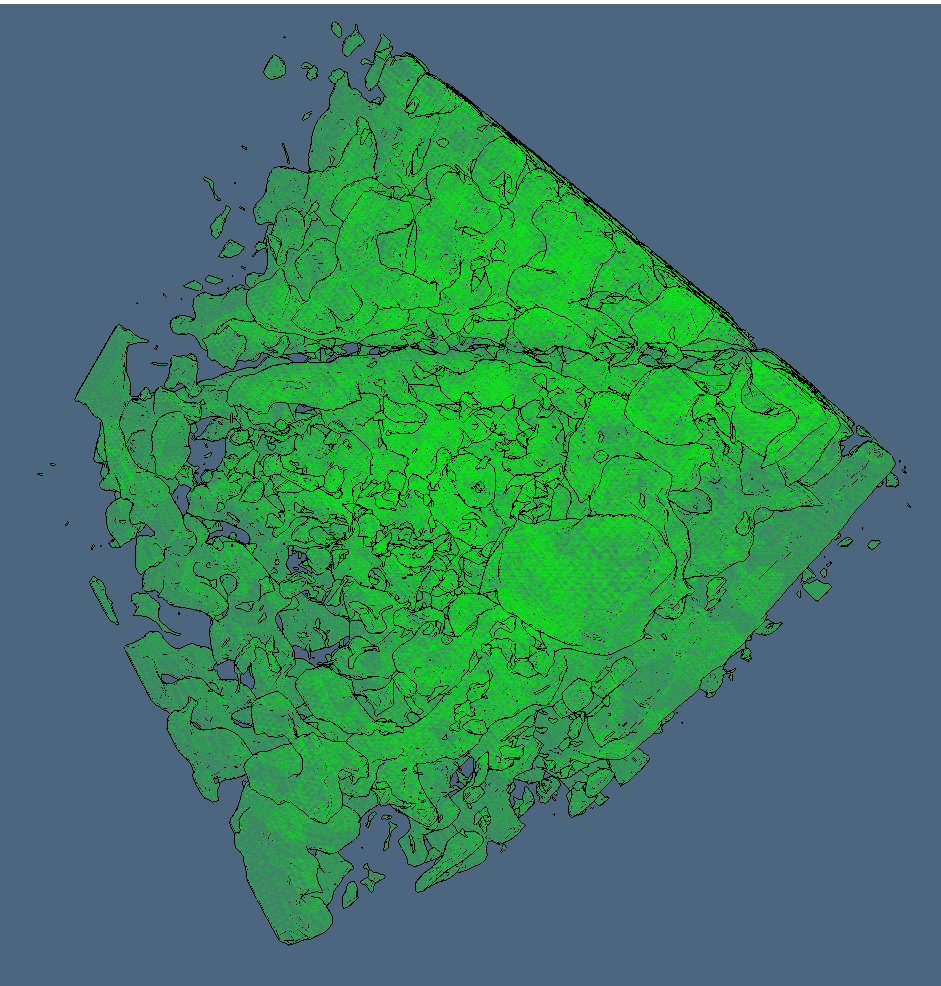
\includegraphics[height=0.3\textwidth]{figs/nrn10_100_green.png} 
%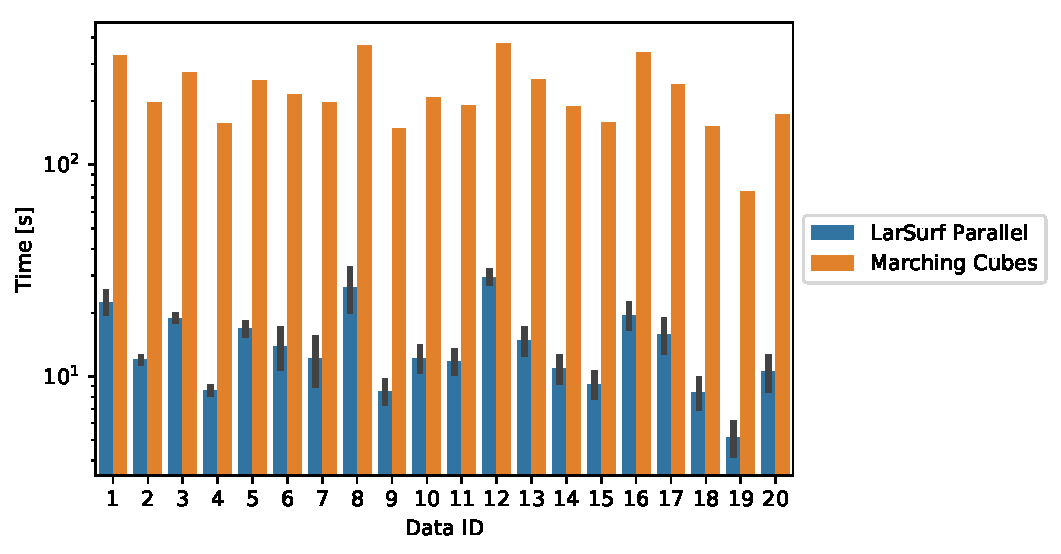
\includegraphics[scale=1]{input/ircad_comparison.pdf} 
\begin{figure}
\centering

\includegraphics[width=0.45\textwidth]{src/figs/ircad01_segmentation_65.png}
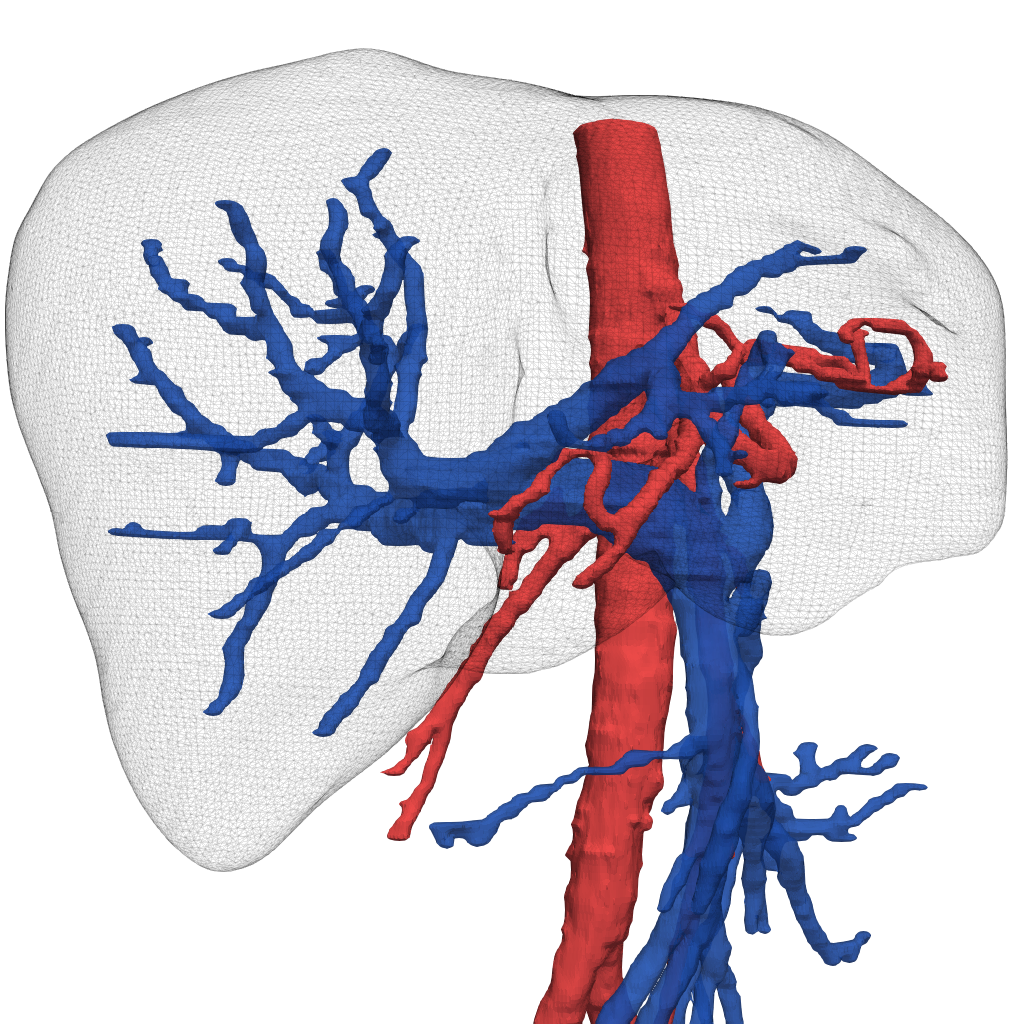
\includegraphics[width=0.45\textwidth]{src/figs/ircad01_liver_tricolore_01.png}
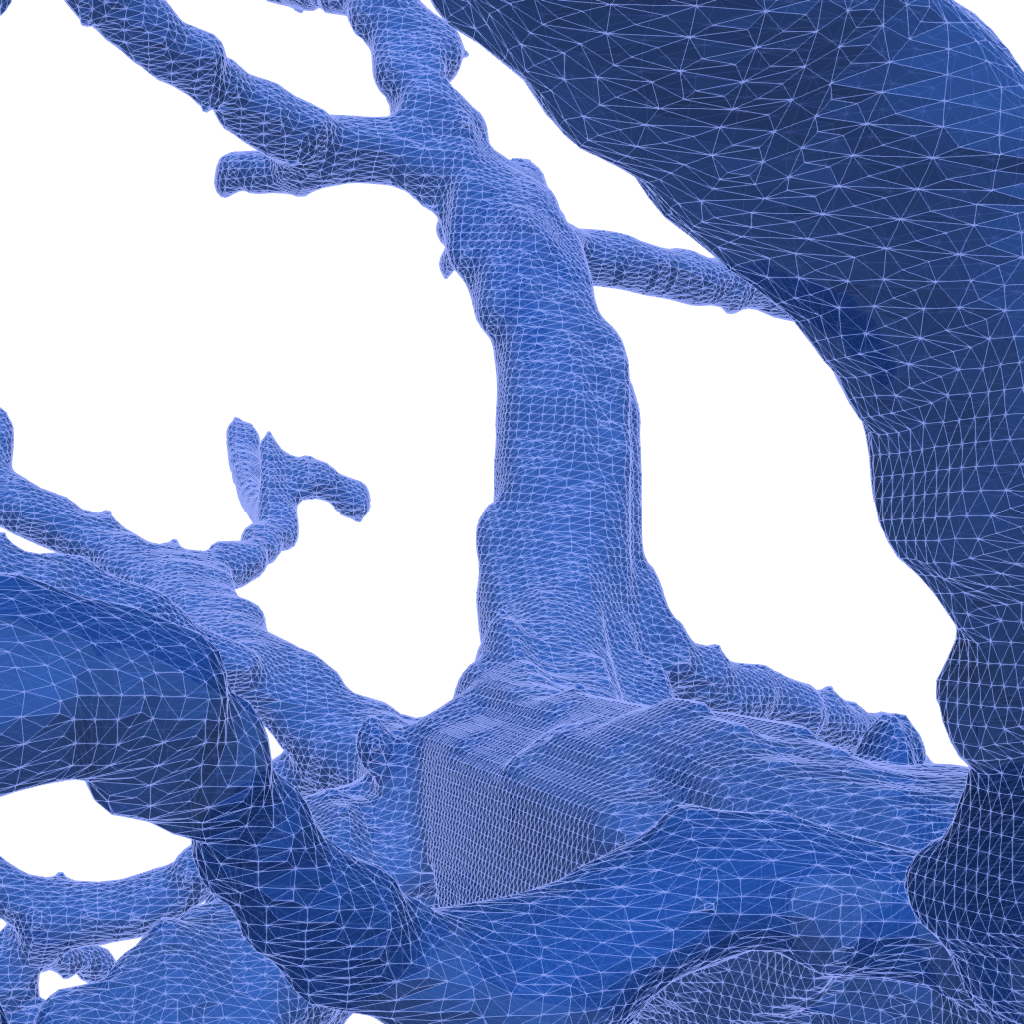
\includegraphics[width=0.45\textwidth]{src/figs/ircad01_porta_blue_01.png}
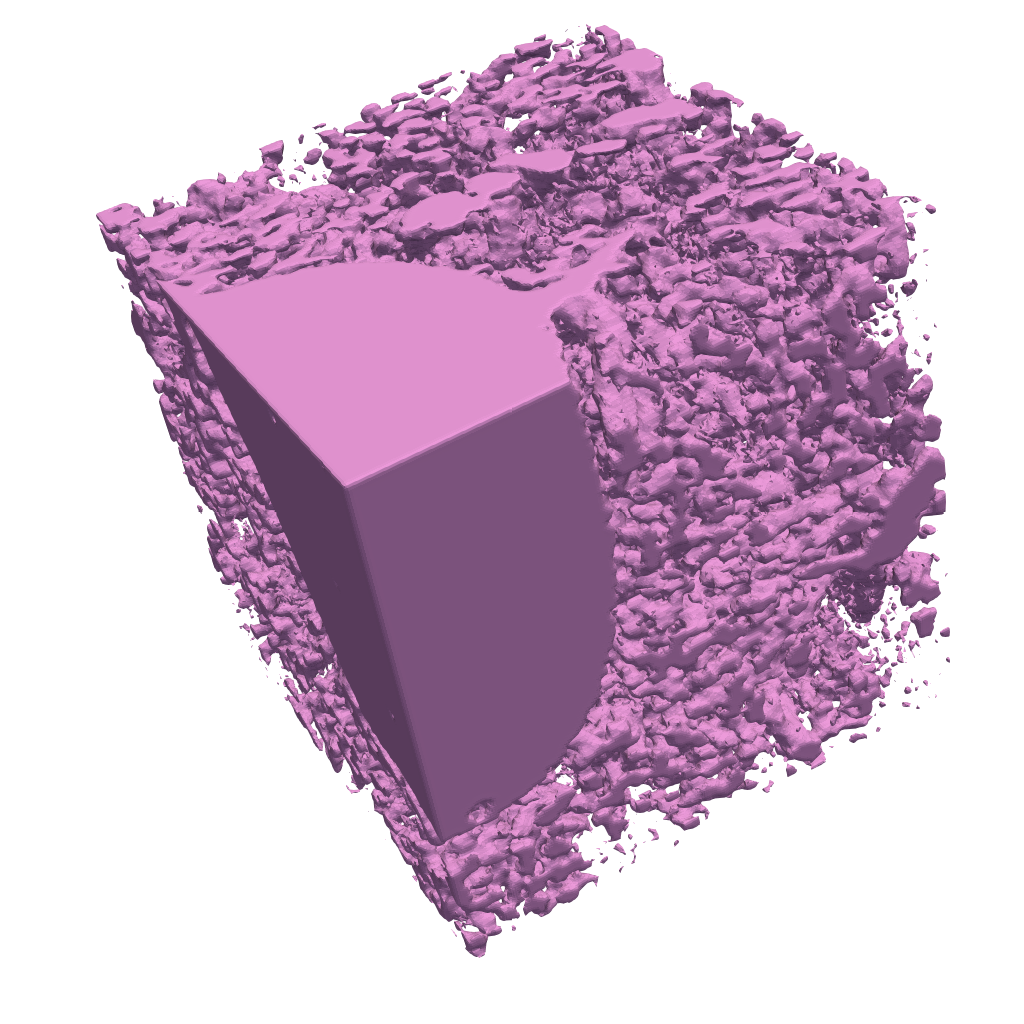
\includegraphics[width=0.45\textwidth]{src/figs/nrn10_200_pink_02.png}
% 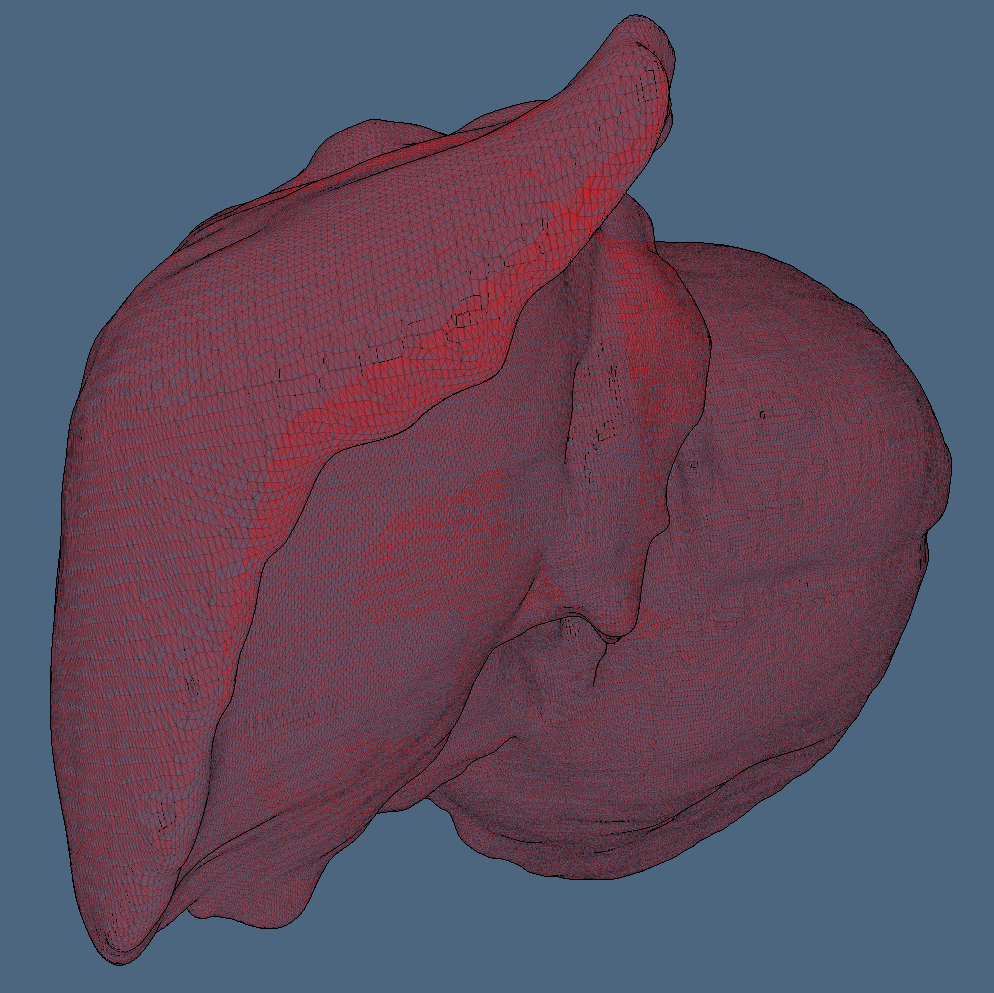
\includegraphics[width=0.4\textwidth]{figs/liver_01_red_3.png} 
% % \vspace{0.05\textwidth}
% 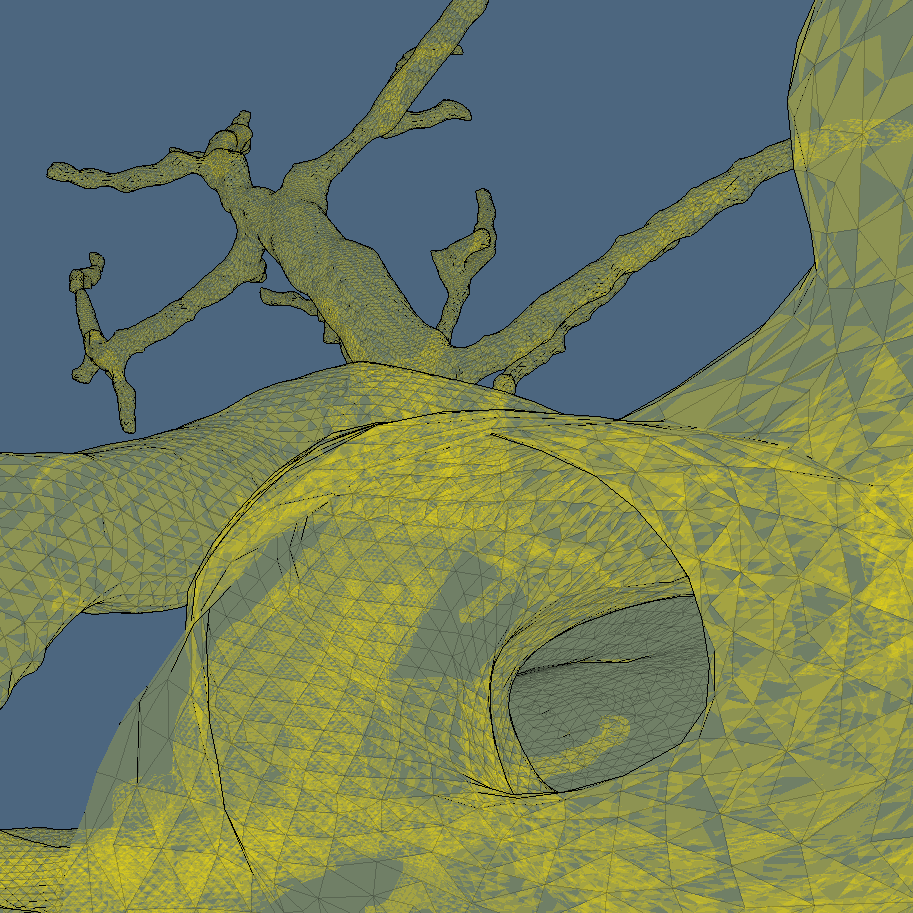
\includegraphics[width=0.4\textwidth]{figs/portalvein_01_yellow_3.png} 
% % \vspace{0.01\textwidth}
% 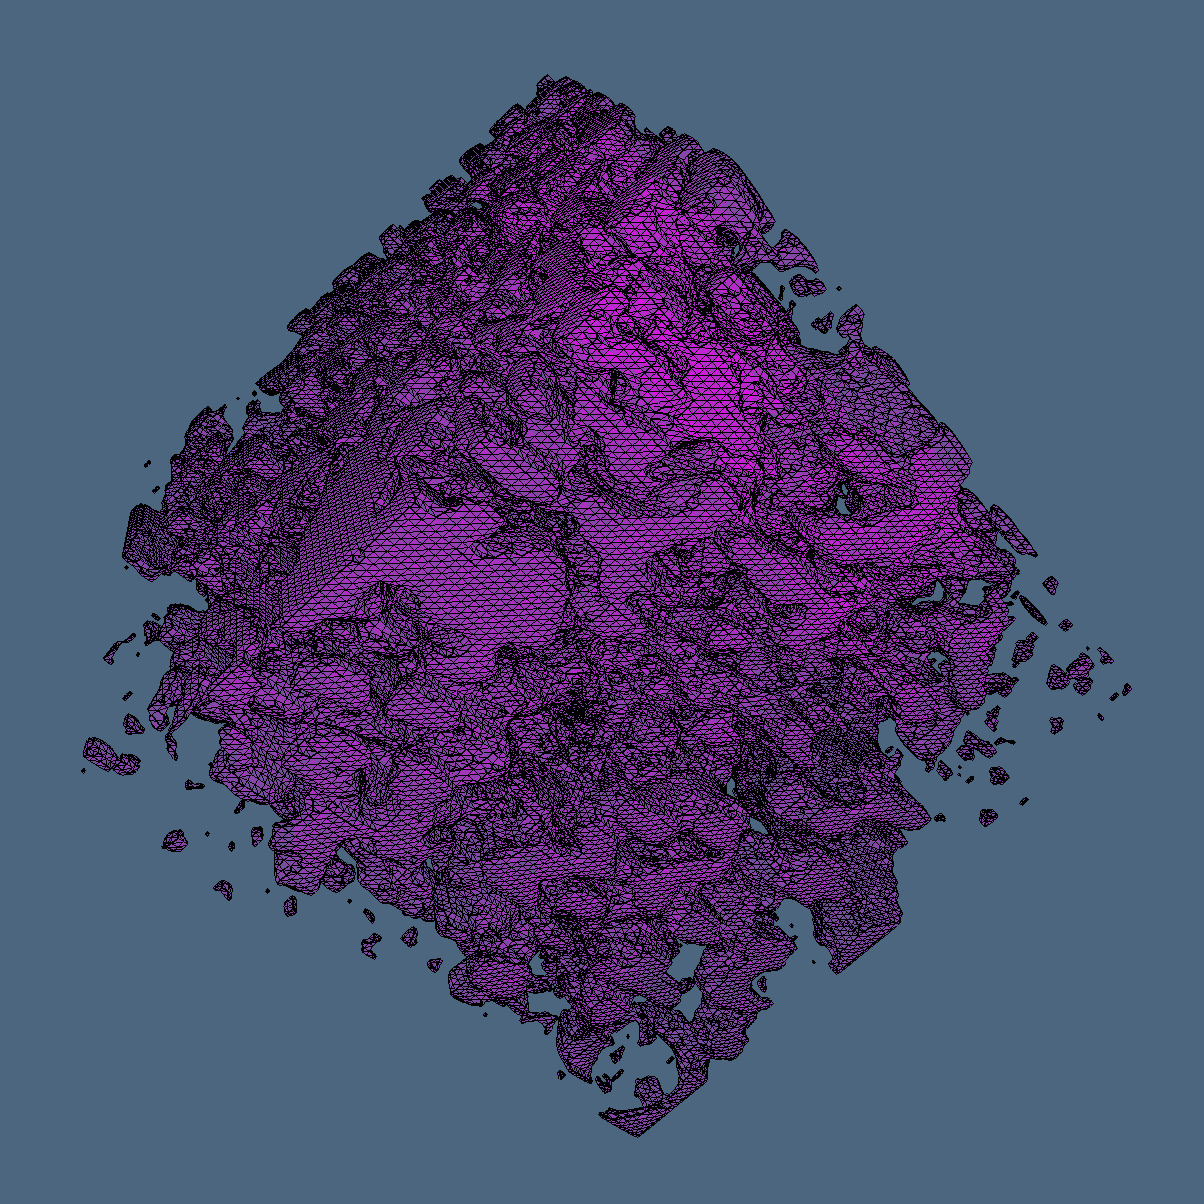
\includegraphics[height=0.4\textwidth]{src/figs/nrn10_100_magenta_high_res.png} 
% % 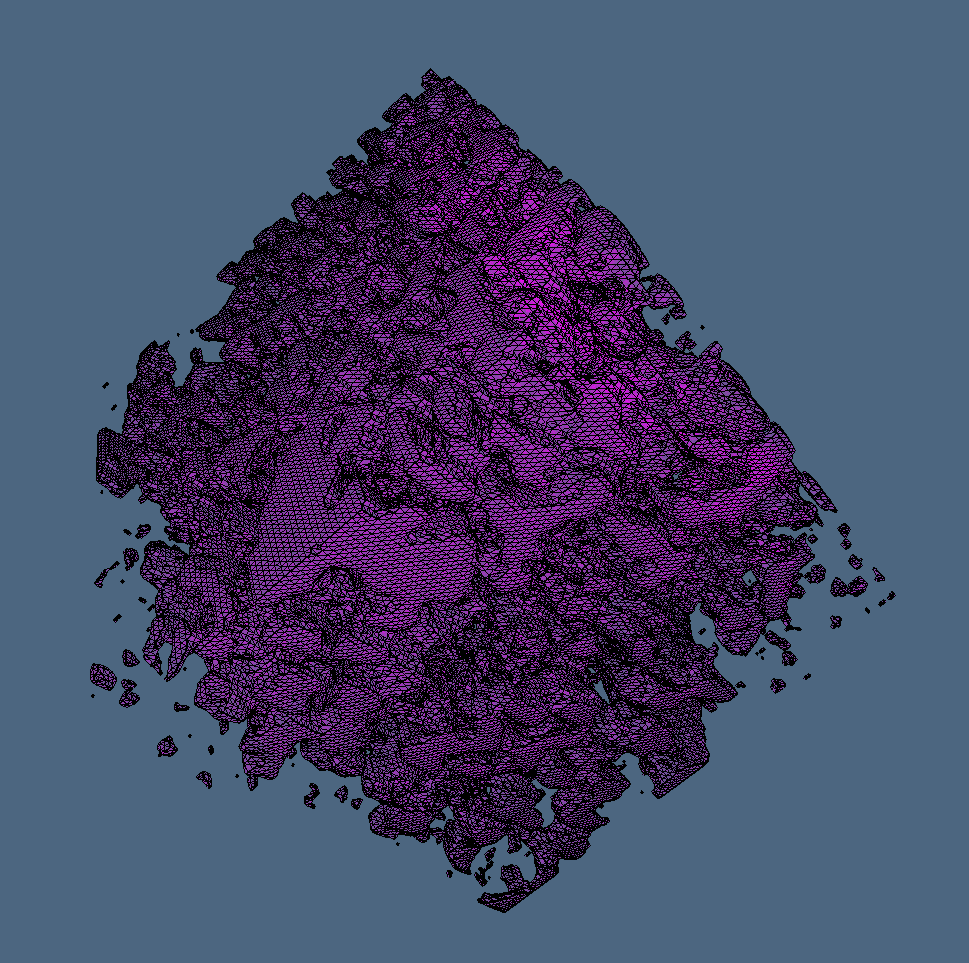
\includegraphics[height=0.4\textwidth]{figs/nrn10_100_low_res.png} 
% % \vspace{0.05\textwidth}
% 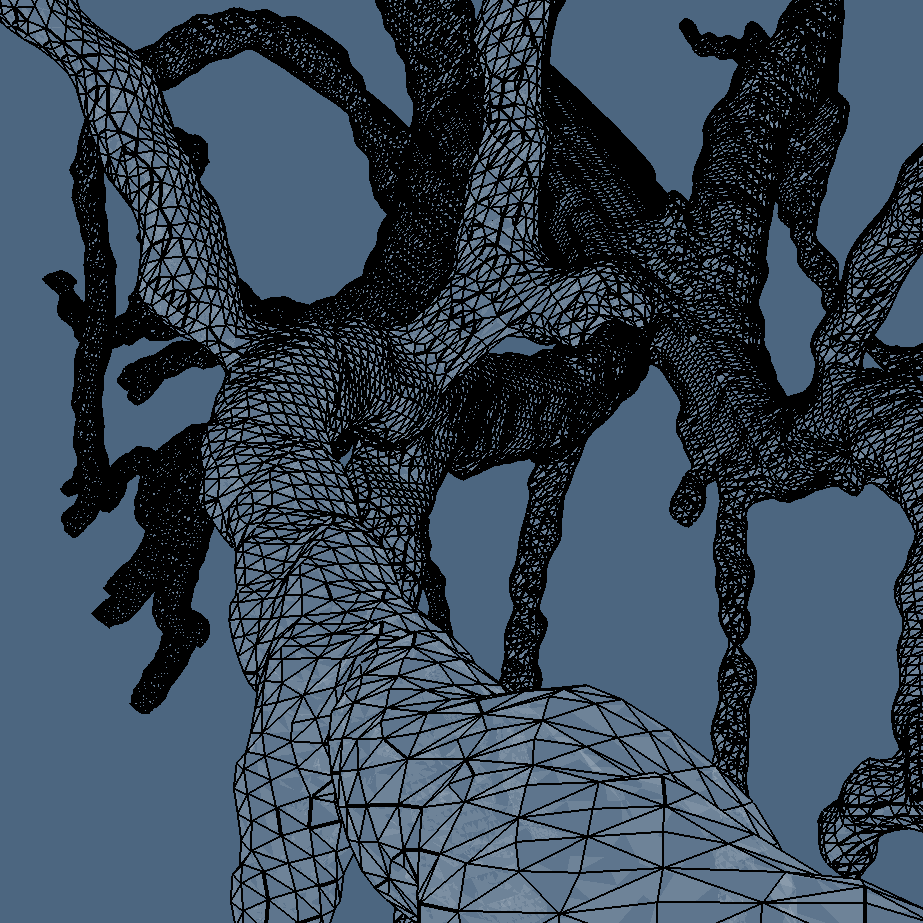
\includegraphics[width=0.4\textwidth]{figs/porta_smoothing_2.png} 
\caption{
Liver structures. The upper left image shows one slice  with segmented organs from  the Ircad dataset \cite{ircad}.
The other images show the triangulated isosurfaces of the macroscopic and microscopic strucures of the liver extracted with \textsc{lar-surf} algorithm. 
On the upper right image can be seen the wire frame model of the human liver along with portal vein and hepatic artery. 
% Both right images show the Portal Vein from the same Ircad dataset \cite{ircad} 
The left bottom image shows the detail of the portal vein  
with resolution $1.6\times0.57\times0.57$ $[mm]$.
On the bottom right image is shown the microvasculature of a pig liver based on corrosion cast prepared by Eberlova
\cite{eberlova2017use}. The size of the speciment is 0.936 $[mm]$ along each axis and the resolution of the Micro-CT data is 4.682 $\mu{}m$.
} \label{fig:example_liver_macro_micro}
\end{figure}

% \begin{figure}
% \centering
% 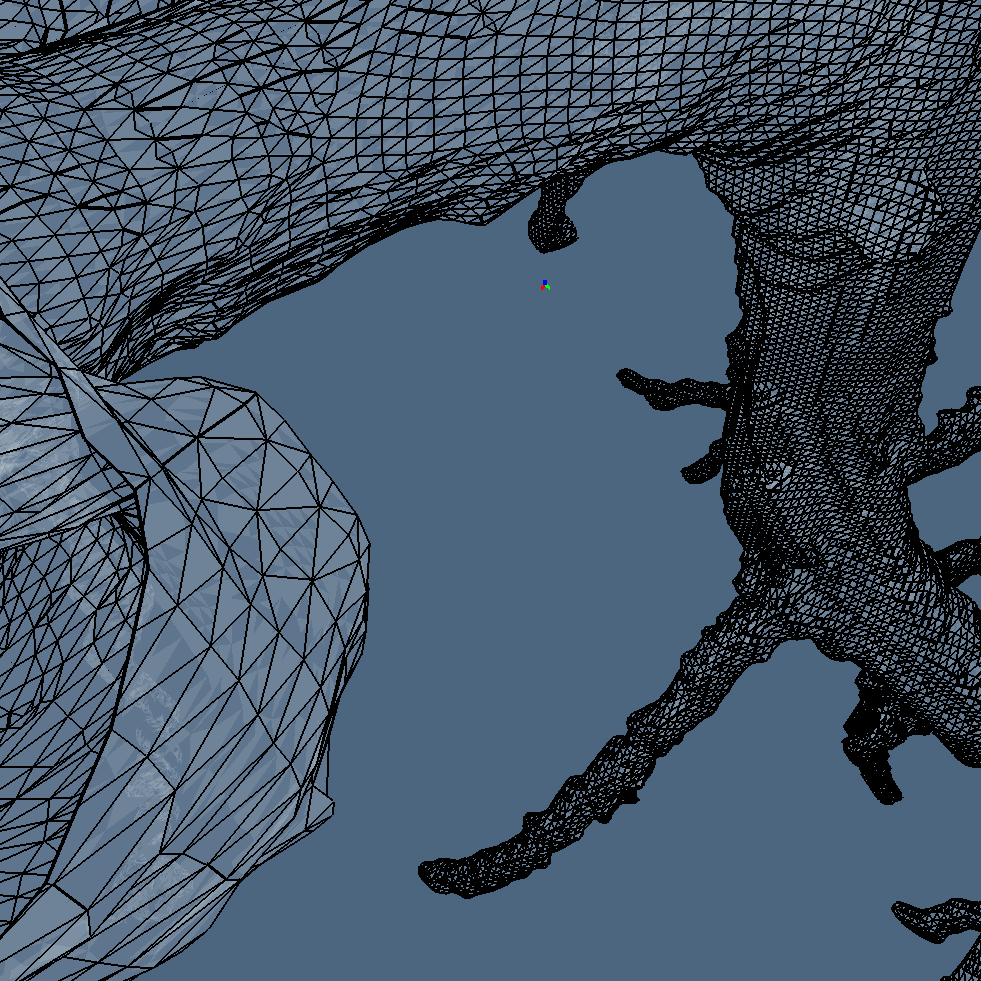
\includegraphics[width=0.4\textwidth]{figs/porta_smoothing_1.png} 
% \vspace{0.05\textwidth}
% 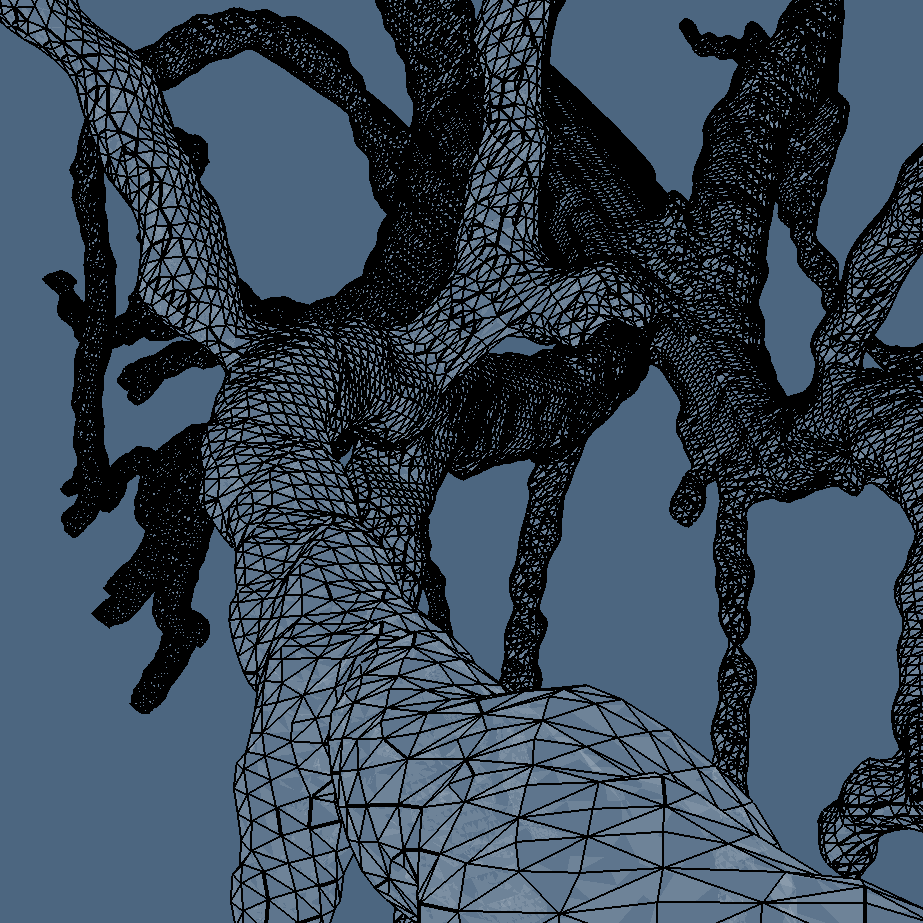
\includegraphics[width=0.4\textwidth]{figs/porta_smoothing_2.png} 
% %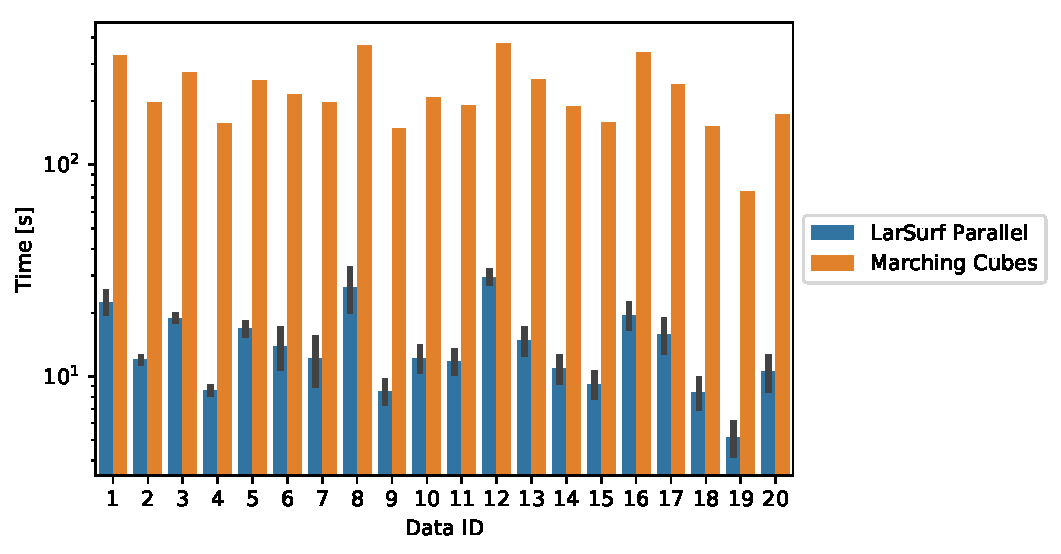
\includegraphics[scale=1]{input/ircad_comparison.pdf} 
% \caption{Triangulated isosurface of portal vein calculated with LAR-SURF}
% \label{fig:example_porta}
% \end{figure}

The implementation of our algorithm is available in LarSurf package. 
Use of this package can be seen on listings \ref{lst:example1} where the liver segmentation with 2865131 voxels from
Ircad dataset is used as an input for our surface extraction algorithm. The size of 3D volumetric 
image is $129 \times 512 \times 512$
and the voxel resolution is $1.6\times0.57\times0.57$ [mm]. 
The output surface model created by  182124 triangles and the number of vertices is 90822. The visualization can 
be seen on figure \ref{fig:example_liver_macro_micro}. 
The portal vein surface extraction can be performed with a small change of input path in code.
The The 3D image resolution is the same. 
It can be seen in the same figure. 
The number of input voxels is 103533. 
The output surface is created by 90822 vertices and 182124 triangles. 

\begin{lstlisting}[caption={Get surface from DICOM volumetric data}, label={lst:example1}]
using Distributed
using Pio3d  # Read 3D data from DICOM files
addprocs(3)  # set number of processors
using LarSurf

LarSurf.lsp_setup([64, 64, 64])  # set block size

# read data from DICOM files
datap = Pio3d.read3d("3Dircadb1.1/MASKS_DICOM/liver")
segmentation = datap["data3d"]
voxelsize_mm = datap["voxelsize_mm"]

# get surface
V, FV = LarSurf.lsp_get_surface(segmentation, voxelsize_mm)
FVtri = LarSurf.triangulate_quads(FV)

# do smoothing and save data
Vs = LarSurf.Smoothing.smoothing_FV_taubin(V,FV,0.5,-0.2,40)
objlines = LarSurf.Lar.lar2obj(Vs, FVtri, "liver.obj")
\end{lstlisting}

The right image of figure \ref{fig:example_liver_macro_micro} is surface of a microvasculature of pig liver. 
Volumetric image is based on Micro-CT data of corrosion casts of pig liver.
\cite{eberlova2017use}.
The size of the visualized data is $100\times100\times100$ voxels and size of voxel is 4.682 $\mu{}m$.
The number of of triangles is 
544784 and number of vertices is 272826.

% \begin{minted}{python}



% using Pkg
% \end{minted}
% \begin{minted}[breaklines,escapeinside=||,mathescape=true, linenos, numbersep=3pt, gobble=2, frame=lines, fontsize=\small, framesep=2mm]{julia}
% Your awesome julia code here\end{minted}






\section{Conclusion}\label{sec:conclusion}

% In this paper we have introduced and discussed a Julia implementation of an algebraic filter to extract from medical 3D images the boundary sourface of a specific image segment, described as a 3-chain of voxels. We have shown a good advantage over standard marchin-cubes algorithms. Translations from cartesian indices of cells to linearized indices, and the sparse matrix-vector multiplication are the main computational kernels of this approach. The current implementation employs Julia's channels for multiprocessing, and can be extended to gain a much greater speed-up using hybrid architectures mixing  CPUs and GPUs of last generation. 

% TODO from abstract
We introduced a Julia implementation of an algebraic filter to extract from 3D medical images the
boundary surface of some specific image segment, described as a 3-chain of voxels. Translations from
Cartesian indices of cells to linearized indices, the computation of the sparse boundary matrices, and the
sparse matrix-vector multiplication are the main computational kernels of this approach. We may show
a good speed-up over marching-cubes algorithms. The existing implementation employs Julia's channels
for multiprocessing. Currently, the computational pipeline is being strongly improved to gain a greater
speed-up using native Julia implementation \texttt{CUDA.jl} of Nvidia programming platform 
% TODO cite Besard2017 [7]
, and the Julia's
\texttt{SuiteSparseGraphBLAS.jl} framework 
% TODO cite BULUK 2017 [8] 
for graph algorithms with the language of linear algebra. In
particular, we are extending its use pattern in order to work with general cellular complexes.



\appendix
\section{Appendix}
\subsection{Symbol list}

\begin{description}
\item[$\mathcal{I}$]  three-dimensional medical image
\\[-7mm]
\item[$\ell_1, \ell_2, \ell_3$]  dimensions of image
\\[-7mm]
\item[$\mathcal{S}$]  segment: a subset of voxels from image segmentation
\\[-7mm]
\item[$\mathcal{B}$] 3D image block
\\[-7mm]
\item[$size$] lateral dimension of cubic block $\mathcal{B}$
\\[-7mm]
\item[$n$]	number of blocks $\mathcal{B}$ (jobs) in $\mathcal{I}$
\\[-7mm]
\item[[$\partial_\mathcal{B}$] ]  boundary matrix for block $\mathcal{B}$
\\[-7mm]
\item[$C_p$] linear (vector) space of $p$-chains
\\[-7mm]
\item[$\nu\in C_p$] $p$-chain
\\[-7mm]
\item[[$\nu$]] coordinate representation (binary vector) of  $\nu$
\\[-7mm]
\item[$\E^3$] Euclidean 3-space
\end{description}


\subsection{Definitions}
\begin{description}

\item[Boundary model] Closed manifold surface of the boundary of a solid model
\\[-7mm]
\item[CSC]  Compressed Sparse Column format for sparse matrices
\\[-7mm]
\item[Global coordinates]  Integer linear coordinates of $\mathcal{I}$
\\[-7mm]
\item[Local coordinates] Integer linear coordinates of $\mathcal{B}$
\\[-7mm]
\item[Cartesian coordinates] Integer triples $(i,j,k)$ one-to-one with voxels
\\[-7mm]
\item[Voxels] Individual elements in 3D image (3-cells)
\\[-7mm]
\item[$p$-chain] Formal linear combination of $p$-cells with coefficients in $\{0,1\}$
\\[-7mm]
\item[Coord. repr.]  Binary vector (for $p$-chains) or binary matrix (for chain operators)
\\[-7mm]
\item[Quad]	Geometric quadrilateral; convex polygon with four vertices
\\[-7mm]
\item[Foreground voxel] Individual element of a segment $\mathcal{S}$
\\[-7mm]
\item[Segment]	Subset of voxels resulting from image segmentation
\end{description}

\subsection{Dataset Ircad}

\begin{table}
\begin{tabular}{rrrrrr}
\toprule
 ID &  z-resolution [mm] &  xy-resolution [mm] &  obj. voxels &  size xy &  size z \\
\midrule
  1 &               1.60 &            0.570000 &      2865131 &      512 &     129 \\
  2 &               1.60 &            0.782000 &      1648024 &      512 &     172 \\
  3 &               1.25 &            0.625000 &      2375079 &      512 &     200 \\
  4 &               2.00 &            0.742188 &      1132427 &      512 &      91 \\
  5 &               1.60 &            0.782000 &      2124505 &      512 &     139 \\
  6 &               1.60 &            0.782000 &      1828493 &      512 &     135 \\
  7 &               1.60 &            0.782000 &      1461944 &      512 &     151 \\
  8 &               1.60 &            0.561000 &      3215090 &      512 &     124 \\
  9 &               2.00 &            0.873047 &      1265420 &      512 &     111 \\
 10 &               1.60 &            0.736000 &      1871804 &      512 &     122 \\
 11 &               1.60 &            0.720000 &      1692716 &      512 &     132 \\
 12 &               1.00 &            0.679688 &      3341433 &      512 &     260 \\
 13 &               1.60 &            0.671000 &      2063109 &      512 &     122 \\
 14 &               1.60 &            0.720000 &      1633641 &      512 &     113 \\
 15 &               1.60 &            0.782000 &      1389572 &      512 &     125 \\
 16 &               1.60 &            0.698000 &      2717185 &      512 &     155 \\
 17 &               1.60 &            0.743000 &      2106497 &      512 &     119 \\
 18 &               2.50 &            0.742188 &      1220564 &      512 &      74 \\
 19 &               4.00 &            0.703125 &       583208 &      512 &     124 \\
 20 &               2.00 &            0.808594 &      1359697 &      512 &     225 \\
\bottomrule
\end{tabular}

\label{tab:ircad1}
\end{table}

\begin{table}
\begin{tabular}{lrrrrr}
\toprule
{} &  z-resolution [mm] &  xy-resolution [mm] &   obj. voxels &  size xy &      size z \\
\midrule
% count &           20.00000 &           20.000000 &  2.000000e+01 &     20.0 &   20.000000 \\
min   &            1.00000 &            0.561000 &  5.832080e+05 &    512.0 &   74.000000 \\
mean  &            1.77750 &            0.725141 &  1.894777e+06 &    512.0 &  141.150000 \\
50\%   &            1.60000 &            0.739094 &  1.760604e+06 &    512.0 &  127.000000 \\
% std   &            0.60273 &            0.077233 &  7.206126e+05 &      0.0 &   44.088756 \\
% 25\%   &            1.60000 &            0.693422 &  1.382103e+06 &    512.0 &  121.250000 \\
% 75\%   &            1.70000 &            0.782000 &  2.187148e+06 &    512.0 &  152.000000 \\
max   &            4.00000 &            0.873047 &  3.341433e+06 &    512.0 &  260.000000 \\
\bottomrule
\end{tabular}

\label{tab:ircad2}
\end{table}

\clearpage{}
\bibliographystyle{alpha}
\bibliography{library,TSAS-2019}

\end{document}
